\InputIfFileExists{ztex_intro-cfg.tex}{}{}
\documentclass[
  hyper, lang=cn,
  mathSpec={envStyle=leftbar},
]{../../zlatex/code/ztex}
\ztexset{
  toc={
    column  = 2,
    title   = 总目录,
    stretch = 1.3
  }
}
\zcolorset{
  % link        = teal,
  definition  = blue
}
\usepackage{enumerate}
\usepackage[bottom]{footmisc}
\usepackage{texhigh}
% \SetKeys[texhigh/high]{config-file=texhigh.cfg}
\SetKeys[texhigh/high]{use-ctab=latex3, lexer-catcode*={0}{}{@=11}}
\ExplSyntaxOn\makeatletter
\cs_set_protected:Npn \__texhigh_env_init:
  {
    \sloppy \hbadness\@M
    \dim_set:Nn \parindent { 0pt }
    \linespread{1.3} \selectfont
  }
\NewDocumentCommand\TikZ{}{Ti\textcolor{orange}{\textit{k}}Z}
\NewDocumentCommand\zTikZ{}
  {
    \ztool_scale_to_wd_and_ht:nnn {.9ex}{1.3ex}{
      \ztool_rotate:nn {89}{\(\aleph\)}
    }\kern-0.3423ex\hbox{\TikZ}
  }
\let\ztikz\zTikZ
\newcommand{\file}[1]{\texttt{\tl_to_str:n {#1}}}
\makeatother\ExplSyntaxOff
% print macro
\let\cmd\ztexverb
\newcommand{\Footnote}[1]{\stepcounter{footnote}\footnote[\thefootnote]{#1}}
\ztexframe[gray]{leftbar}
\def\meta#1{\ensuremath \langle #1\ensuremath \rangle}
\newcommand{\zkey}[1]{\texttt{\meta{#1}}}
\newcommand{\pkg}[1]{\textsf{#1}}
\newcommand{\cls}[1]{\textsf{#1}}
\def\lrr#1{\ensuremath{\Rightarrow}}
\AddToHook{cmd/section/before}{\thispagestyle{plain}}


\title{z\TeX{} Bundle}
\author{Eureka}
\date{\today}

\begin{document}
% cover
\ExplSyntaxOn
\zpagemask[position={(0pt, .25\zph)}, anchor=l]{
  \rlap{\color{gray!25}\rule{\zpw}{6em}}
  \hcoffin_set:Nn \l_tmpa_coffin {\sffamily\Large\color{black!75} 由于本人时间有限, 目前此宏集的开发暂停.}
  \coffin_typeset:Nnnnn \l_tmpa_coffin {hc}{vc}{.5\zpw}{3em}
}
\ExplSyntaxOff
\maketitle
\thispagestyle{empty}
\tableofcontents
\clearpage


\section{简介}
\subsection{为何叫 z\TeX{}?}
为什么宏集名称里面有 `z' 这个前缀, 这也许应是许多用户想知道的问题 ? 下面是可能的几点原因:

\begin{enumerate}[(1)]
  \item 看到 \LaTeX3 开发团队用 ``x'' 来作为他们开发的一系列宏包前缀,比如 \pkg{xparse}, \pkg{xcoffins}, \pkg{xfp} 等。
    我便不能再使用 ``x'' 这一前缀了. 这个时候, 突然想到了一个字母 -- ``z''. 一方面 ``x → y → z'', 有了``x'', 才有 ``z''
    (\zTeX{} 全部基于 \LaTeX3 进行开发; 可以说,没有 \LaTeX3, 就没有今天的 \zTeX{}). 那么 ``y'' 去哪里了 ? 当作为用户的你 (you) 
    加入 \zTeX{} 使用者阵营后, 就有 ``y'' 了.
  \item 你将 `z' 逆时针旋转 90$^\circ$, 就可以得到 ``阿列夫 -- $\aleph$'': 我希望 \zTeX{} 宏集能够有进一步(无限)拓展的可能;
    这个宏集在设计之初, 便一直坚持可拓展性这一原则. 普通用户可以使用用户层面的命令, 模板制作者可以使用 \ztex{} 提供的编程
    接口. 尽管 ``$\aleph$\TeX'' 这个目标有些不切实际, 但是万一实现了呢 ?
  \item 也许是看到了 \TikZ{} 中的 ``z'', 于是便以 `z' 为本系列宏集的前缀了 .
\end{enumerate}

最开始的 \ztex{} 宏集仅包含一个基本的 \cls{zlatex.cls} 文档类, 而且原来的名称叫做 ``$\pi$\LaTeX{}"; 后面我又想基于 \TikZ{} 
开发一个绘图宏包, 用于实现常见平面图形的绘制以及外部程序的交互; 再后来发现 beamer 用起来很不方便, 便开发了 \pkg{slide} 库;
随着开发的不断深入, 我发现我已经在 \cls{ztex.cls} 中写了很多十分有用的宏了, 于是我把这些宏分化了出来, 得到了 \pkg{ztool} 宏包,
得到了 \pkg{thm}, \pkg{cmd}, \pkg{font}, ... 这些模块, 以及 \pkg{slide}, \pkg{alias}, \pkg{thm} ... 这些库; 最终, 
\ztex{} bundle 诞生了.


\subsection{为何用 z\TeX{}?}
为什么要用我这个 \ztex{} 宏集 ? \zTikZ{} 中负责和外部程序交互的那几个模块现在处于一种比较尴尬的境地, 用户如果会用
这些程序, 那么你可以单独使用这些程序调整图片的所有细节, 最后在 \LaTeX{} 中插入该图片. 如果用户不会使用这些外部拓展程序,
那么用户不仅需要先学习该程序的用法, 还需要学习 \zTikZ{} 宏集中对应命令的 \LaTeX{} 语法; 这无疑是增加了用户的负担 !

用户可以再思考这样一个问题: 我已经会用 \LaTeX{} 自己写模板了, 为什么还要用别人的模版 ? 我如果不会用 \LaTeX{} 写模板,
花费了大量的时间去了解一个庞大且复杂的模板的使用细节, 那么我为何不花费这些时间自己去学习 \LaTeX{}, 这样更能做出满足自己需求的模板 ? 
最后还可以进一步推出: 我为什么一定要用 \TeX{} 或 \LaTeX{} 呢 ? 用 Word, Indesign 这些成熟的软件, 甚至是手写, 难道就不能写一篇
规范的论文/笔记吗 ? 

所以为什么 Knuth 老爷子要花费十年的时间去开发 \TeX{} 呢 ? 

上述的一系列推论正确吗 ? 仔细想一想, 上面的推导其实不都是正确的. 前一个条件并不一定是充分的, 或者说我们使用了一个
假命题(关系)去得到了另一个命题(关系). 

根据基础的逻辑知识: 定义汇集 $\text R \vee \text S$ 为两关系 R, S 的逻辑析取, 定义汇集 $\lnot \text R$ 为关系 R 的逻辑否定. 
从而我们就可以定义所谓的 ``逻辑蕴含'' 关系 $\lrr{}$, 即记号 $\text R\lrr{} \text S$, 前者其实是如下的关系汇集:
\[
  \text S \vee (\lnot \text R)
\]

\begin{remark}
其实有 $\lnot, \vee$ 这两个基础的符号就已经能表示出很多的关系了; 比如逻辑合取记号: $\text R\wedge \text S$, 它其实就是:
$ \lnot [(\lnot \text R)\vee (\lnot \text S)]$. 在规定逻辑公理后, 就可以用它们来说明常用的 ``三段论, 双重否定'' 等
逻辑推理了. 比如我们常用的逆否命题就是说: 关系 $(\text R\lrr{}\text S) \lrr{} ((\lnot\text S)\lrr{}(\lnot\text R))$
是真的.
\end{remark}

在我们定义了关系 ``真'' 后, 如果关系 $\text R\lrr{}\text S$ 是真的, 那么:
\begin{itemize}
  \item 当关系 R 为真的, 关系 S 必然是真的, 也就是我们得到了一个 ``真'' 的结论;
  \item 但如果 R, S 同时为假, 关系 $\text R\lrr{}\text S$ 也是真的. 而此时我们的结论并不是 ``真的'', 
    也就是结论并不成立.
\end{itemize}

可以认为我们用一个假命题导出了另一个假命题, 下面说明 \zTeX{} 值得你去用, 我将要如何去说服你呢 ? 


让 ``R\; \lrr{} S'' 中的命题 ``R'' 为假就好了. \ztex{} 的上手难度相较于默认的 \LaTeX{} 要低一点, 达到
同样的排版效果, 你所花费的时间更少. 故上述 ``花费同样时间'' 这一个命题为假, 即 ``z\TeX{}值得你用'' 这一命题成立.
你也许可以用其它的方式来反驳我, 但至少我找到了一个论据来说服我自己, 也找到了我开发这个宏集的初心.

\subsection{项目维护}
目前本项目已经在GitHub, Gitlab, Gitee上开源, 地址如下:

\hspace*{6em}\parbox{\textwidth}{
\begin{itemize}
  \item [GitHub]: \href{https://github.com/zongpingding/zTeX_bundle}{https://github.com/zongpingding/zTeX\_bundle}
  \item [Gitlab]: \href{https://gitlab.com/zongpingding/zTeX_bundle}{https://gitlab.com/zongpingding/zTeX\_bundle}
  \item [Gitee] : \href{https://gitee.com/zongpingding/zTeX_bundle}{https://gitee.com/zongpingding/zTeX\_bundle}
\end{itemize}}

项目中包含: \cls{ztex} 文档类, \zTikZ{} 宏包, 以及 \pkg{ztool} 宏包的源码与用户手册. \ztex{} 宏集以 lppl 协议开源, 欢迎各位
对源代码进行修改与二次分发. 若用户在使用此宏集的过程中发现任何的 Bug, 或想提出改进意见, 请在 Github 上提 Issue 或直接提交 PR. 


请不要在 Gitee 或者是 Gitlab 上提问, 本人只维护 Github 上的仓库; 尽管有时可能会为了国内用户下载方便, 把 Github 仓库中的内容同步到
这两处. 后续的开发过程中, 三者不会同步更新, 请以 Github 仓库为准.

本项目为完全免费、纯属兴趣驱动(为爱发电)之作。对于任何使用本模板所引发的严重后果,我概不负责。
我非常乐意帮助大家解决问题,但在提问之前,请务必先了解 \LaTeX{} 的提问规范,让我们共同营造一个友好、愉快的交流氛围.

当前宏集的稳定版本于半年之前发布, 最新的开发版请切换到 ``dev'' 分支; 本手册适用于当前最新的开发版.
请到: \href{https://github.com/zongpingding/zTeX_bundle/releases}{Release 界面} 下载.


\clearpage
\subsection{基本组成}
\ztex{} 宏集包含如下内容:
\begin{multicols}{2}
  \begin{itemize}
  \item \cls{ztex} 文档类;
  \item \pkg{ztool} 宏包;
  \item \pkg{ztikz} 宏包;
  \item \pkg{zslide} 宏包(不推荐使用).
\end{itemize}
\end{multicols}

\ztex{} 宏集独立实现了一个 \pkg{ztool} 宏包, 它是 \ztex{} 宏集中各文档类或宏包的基础. 此宏包中包含原来已被废弃
的 \pkg{l3sys-shell} 中的所有命令. 除此之外, \pkg{ztool} 提供了 box 操作, 文件 IO 以及基本图形绘制相关的函数. 
在 \pkg{ztool} 的协助下,\ztex{} 能够避免或减少命令行 \cmd{-shell-escape} 参数或其它相关宏包的调
用(如 \pkg{robust-externalize} 宏包).

\cls{ztex} 文档类对标 \cls{memoir}, \cls{koma-script} 宏集, 用于生成书籍或演示文稿.
尽管在 \ztex{} 中, 直接将 \cmd{layout/slide} 选项置为 \texttt{true} 即可生成演示文档, 但该库目前很不成熟荐使, 
所以在严肃场合中, 推荐使用原始的 \cls{beamer} 或 \cls{ctexbeamer} 文档类.

\zTikZ{} 宏包提供了绘制平面图形以及调用外部程序的接口\Footnote{众所周知的, 在 \LaTeX{} 中绘图是一件十分痛苦的事情,
于是乎你会看到很多书籍或笔记中的图形都是手绘或截图, 并非矢量图}. \pkg{zslide} 宏包是自己临时设计的一套 beamer 主题, 还未进行常规测试, 
请谨慎使用.


从本介绍文档即可看出,本模板整体风格较为朴素,未采用华丽的配色方案或精致的页面设计。然而,在长时间尝试和调试 \LaTeX{} 模板的过程中,
我逐渐发现这种简洁质朴的风格最符合广大 \LaTeX{} 用户的使用习惯与审美偏好. 若你更倾向于精美的排版风格,亦可参考其他的模板,如 
\href{https://github.com/ElegantLaTeX}{Elegant\LaTeX{}}、
\href{https://github.com/BeautyLaTeX/Beautybook}{Beauty\LaTeX{}} 等.


\subsection{用户手册}
普通 \LaTeX{} 用户可跳过本文档的 ``\cref{模板设计}''. 该部分主要记录了我对本模板设计思路的说明,以及个人
在编写 \LaTeX{} 过程中的一些体会,对模板或宏包的实际使用并无直接帮助。若你希望了解 \cls{ztex} 文档类的具体用法,
请参阅 \file{zlatex_interface.pdf}; 若需了解 \pkg{ztikz} 宏包的使用方法,请参阅 \file{ztikz_interface.pdf}.
目前 \pkg{zslide} 宏包尚无详细文档,仅提供了示例文件 \file{zslide_manual.pdf} 供用户参考. \pkg{ztool} 宏包 
主要为模板的开发者准备, 普通用户无需阅读.


\newpage
\section{安装使用}
\subsection{在线模板}
为了让部分用户可以直接使用到 \ztex{},免去``繁杂''的环境配置. 我已将本模板部署在 \TeX{}Page 上,
地址为: \href{https://www.texpage.com/share/e420ac8364a640b78231d65c9d5d7090}{TeXPgae \ztex{}  Project},
直接打开此地址即可体验. 由于技术原因,\zTikZ{} 请在本地体验.


\subsection{本地安装}
\ztex{} 宏集目前还未上传 CTAN, 因为还没有开发完成. 本文档类使用的部分
\LaTeX3 命令在老版本的 \TeX{}Live 下并不存在, 若用户的 \TeX{}Live 版本过低,则可能无法正常使用本宏集. 
目前 \ztex{} 文档类在各平台的兼容情况为:

\hspace*{12em}\parbox{8cm}{
\begin{itemize}
  \item[Windows]: \TeX{}Live 最低版本 2025
  \item[Linux]: \TeX{}Live 最低版本 2025
  \item[MacOS]: Mac{}\TeX{} 还未测试
\end{itemize}}

因 \ztex{} 还未传入 CTAN(未来可能会考虑), 所以想要使用此文档类,只有如下两种方法:
\begin{itemize}
    \item 把此宏集 -- \file{ztex} 目录中的所有内容放入当前项目文件夹下;
    \item 在命令行运行命令: \file{kpsewhich -var-value=TEXMFHOME}, 在 Windows 上这个路径一般是: \texttt{C:/Users/\meta{name}/texmf/}, 
      在Linux下一般是: \file{~/texmf/}; 具体路径以自己的实际情况为准. 在此路径下新建文件夹 \file{tex/latex/ztex}; 此文件夹对应的路径
      我们记为 \meta{z\TeX}, 随后把 \file{ztex} 目录中的所有内容放入 \meta{z\TeX} 下即可.
\end{itemize}

在本手册后续,我们使用 \meta{z\TeX} 表示本宏集的根目录.

\vskip1.5em
\noindent{\color{red}\sffamily NOTE: 如果用户不需要使用 \pkg{alias} 库, 那么一些比较老 \TeX{}Live 也能运行此宏集.}



\clearpage
\section{开发过程}\label{模板设计}
本模板的设计经历了较长时间的积累与迭代。最初接触 \LaTeX{} 时,我只是将常用的宏整理进一个 \file{.sty} 文件中,误以为这便是一个宏包
(实际上它称得上是一个宏包). 随后接触到了 \href{https://github.com/ElegantLaTeX}{Elegant\LaTeX{}} 系列模板,并曾使用其中的 
\cls{elegantbook} 文档类撰写笔记。然而,随着使用深入,我逐渐发现模板默认的样式并不完全符合个人需求,许多细节希望能够自行定制。
遗憾的是,当时对 \LaTeX{} 的理解尚浅,面对复杂的模板源码无从下手(打开任何一个模板, 映入眼帘的源码对于我来说与一堆乱码无异)。
后续通过查阅资料、阅读相关文章,逐步积累经验,渐渐熟悉了 \LaTeX{} 中的各种命令与机制,才最终开始着手本模板的独立设计.

\ztex{} 的第一版基本是在 \cls{elegantbook} 文档类的基础上修改而成,仅在字体、配色等方面做了一些简单调整。然而,
随着功能的不断叠加,模板逐渐变得混乱,代码结构也变得难以维护\Footnote{事实上,最初 \ztex{} 与 \pkg{ztikz} 
宏包是写在一起的,整体结构非常凌乱.}。其中,键值对接口的实现对于我来说尤为困难。以文档类语言切换功能为例, 当时通过 \cmd{\ifdefstring} 
实现,以下是当初的相关代码片段:


\begin{texhigh}[]
\DeclareVoidOption{cn}{\kvs{lang=cn}}
\DeclareVoidOption{en}{\kvs{lang=en}}
\DeclareStringOption[cn]{lang}
\end{texhigh}

代码的书写过程颇为繁琐。当时模板仍以 \cls{article} 文档类为基础,缺乏许多 \cls{book} 文档类中内置的计数器与章节结构,不得不自行声明相关命令。
然而,自定义的命令常与其他宏包不兼容,尤其是在集成 \pkg{hyperref} 宏包时问题频出。由于计数器定义不规范,导致跳转功能异常。例如,
使用 \cmd{\label} 时,所激活的跳转目标往往并非正确的章节位置,目录中的链接也存在类似问题,使用体验大打折扣。

另一方面,初代 \ztex{} 文档类完全基于 \LaTeX{}2$\varepsilon$ 构建,许多宏展开相关的代码写的不仅繁琐,逻辑
也很混乱。当时经验有限,模板中的大多数解决方案都借鉴(抄袭)自 \href{https://tex.stackexchange.com/}{\TeX-StackExchange} 
上的回答,导致整个模板虽然 ``能跑'',但对其中许多命令的具体作用并不真正理解, 并不清楚这些 ``解决方法'' 会不会产生一些不为人
知的副作用.



\clearpage
\subsection{\texorpdfstring{\zTeX{}}{zTeX} }
后来,我将 \pkg{ztikz} 宏包从原有的 \cls{ztex} 文档类中剥离出来,并使用 \LaTeX{}3 对原始文档类和 \pkg{ztikz} 进行了重构。
\ztex{} 文档类默认基于 \cls{article} 文档类构建,同时也支持加载其他文档类。此阶段的开发理念发生了显著变化: 在添加任何的配置前,
我都会事先明确其提供的功能, 了解该配置需要的依赖, 这一配置对已有的代码或宏包有无影响, ..., 然后再自行编写代码实现。由此,z\TeX{} 的开发正式开始了.
事实证明,基于 \LaTeX3 的重构极大提升了代码的清晰度和整体开发效率。以下为当时 \pkg{ztex} 文档类选项的相关声明:

\begin{texhigh}[]
\zlatex_define_option:n {
  % language
  lang             .str_gset:N  = \g__zlatex_lang_str,
  lang             .initial:n   = { en },
  % page layout
  layout           .str_gset:N  = \g__zlatex_layout_str,
  layout           .initial:n   = { twoside },
  % margin option
  margin           .bool_gset:N = \g__zlatex_margin_bool,
  margin           .initial:n   = { true },
}
\ProcessKeysOptions {zlatex / option}
\end{texhigh}

看起来确实清爽了许多,但很快我意识到,这样的实现方式在实际使用中仍不够灵活。问题在于:当需传递给子文档类的选项较多时,
必须逐一声明大量键值对;而当整个文档类中键值对数量庞大时,维护成本显著增加。
为了解决这一问题,我引入了 \pkg{l3keys} 提供的元键机制(\cmd{.meta:nn})。其核心作用在于:通过模块化管理各类键值对,
实现层级式组织与调用,从而提升代码的可读性与扩展性。以下是当时 \pkg{ztex} 文档类中键值接口的实现代码:


\begin{texhigh}[]
\zlatex_define_option:n {
  % zlatex language
  lang            .str_gset:N   =  \g__zlatex_lang_str,
  lang            .initial:n    =  { en },
  % class and options
  class           .str_gset:N   = \g__zlatex_subclass_type_str,
  class           .initial:n    = { book },
  classOption     .clist_gset:N = \g__zlatex_subclass_option_clist,
  classOption     .initial:n    = { oneside, 10pt },
  % zlatex options meta key 
  layout          .meta:nn      = {zlatex / layout}{#1},
  mathSpec        .meta:nn      = {zlatex / mathSpec}{#1},
  font            .meta:nn      = {zlatex / font}{#1},
}
\end{texhigh}

为了轻松处理子文档类选项的加载问题, 我引入了 \zkey{classOption} 这个键. 


\clearpage
\subsection{\texorpdfstring{\zTikZ}{zTikZ}}
开发宏包 \pkg{ztikz} 也花了我很多的时间, \pkg{ztikz} 从最开始的一个小宏包变成了一个拥有众多拓展库的庞然大物.
这段时间, 我为 \pkg{ztikz} 宏包开发了 \pkg{cache}, \pkg{python}, \pkg{gnuplot}, \pkg{wolfram} 和 \pkg{l3draw} 库. 
这些库可以先通过下面的命令进行声明:

\begin{texhigh}[]
\ProvidesExplFile{ztikzmodule.cache.tex}{2024/06/15}{1.0.0}{cache~module~for~ztikz}
\end{texhigh}

\noindent 然后在主宏包 \pkg{ztikz} 中使用如下命令进行调用:
\begin{texhigh}[]
\cs_new_nopar:Npn \g__ztikz_load_module:n #1 
  {
    \clist_map_inline:nn {#1} 
      { \file_if_exist_input:nF {modules/ztikzmodule.##1.tex}{} }
  }
\NewDocumentCommand\ztikzLoadModule{m}
  {
    \g__ztikz_load_module:n {#1}
  }
\end{texhigh}

\noindent 划分出 \pkg{ztikz} 的库后, 宏包使用者只需通过如下的命令就可以轻松调用:
\begin{texhigh}[]
\ztikzLoadModule{cache, python}
\end{texhigh}

而且, 将一个宏包划分为一个个的库来开发这一行为, 不仅可以方便宏包的使用者, 更让宏包的开发
者可以聚焦于单个库的开发, 这极大地提高了我的开发效率.

在开发 \pkg{ztikz} 的 \pkg{cache} 库时, 我遇到了数不清的困难, 包括但不限于:
\begin{itemize}
  \item 怎么将一个环境中的内容不加改变地输出到外部文件中 ?
  \item 怎么为每一个需要缓存的内容 ``打'' 上一个唯一的 ``身份标签'' ?
  \item 为什么同样都是字符串, 但是 string 和 token list 在 \cmd{\tl_if_eq:nn} 中就是判断为不相等 ?
  \item 怎么调用上一次的缓存结果 ?
  \item 怎么临时忽略缓存机制, 或强制调用上一次的缓存结果 ?
  \item 怎么提供对应的编程接口 ?
  \item ...
\end{itemize}

\noindent 虽然, 上述的问题目前均已解决, 但目前的 \pkg{cache} 库仍有缺陷:
\begin{itemize}
  \item 无法去除 \pkg{tikz} 的 \pkg{externalize} 库依赖, 我自己还没有能力自己写一个 \pkg{externalize} 库出来.
  \item 无法提供与 Matlab 的交互接口 .
  \item \pkg{cache} 库提供的普通用户接口仍然过于复杂 .
  \item ...
\end{itemize}


\subsection{ztool}
大概是开发到中后期的时候, 我发现我在 \cls{ztex} 或 \pkg{ztikz} 中定义了大量与此宏包无关的宏, 
比如 ``\TeX{} 盒子操作'', ``shell-escape'', ``文件 IO 操作''; 然后我便把这些宏分离到了 \pkg{ztool} 
宏包中. 上面的这些功能几乎时没有什么关联的, 后面我更是在 \pkg{ztool} 宏包内将它们划分为了下面的这几个部分:
\begin{itemize}
  \item shell-escape,
  \item file-io,
  \item box,
  \item zdraw;
\end{itemize}

它们之间互不干扰, 用户在使用时仅需加载其需要的部分即可; 比如用户需要使用 \pkg{file-io} 中的一个宏,
他只需要使用如下的命令:
\begin{texhigh}[]
\ztoolloadlib{file-io}
\end{texhigh}

\noindent 此时, \pkg{ztool} 仅会加载 \pkg{file-io} 相关的宏, 其它部分的宏则不会被加载. \pkg{ztool}
实现这一机制同样是使用了上述方法 -- 将 \pkg{ztool} 划分为一个个的库.


\clearpage
\subsection{l3build}
我之前完全没有接触过 ``代码测试'' 相关的内容, 一个偶然的时间,我发现了 \pkg{l3build}. 我们写的代码是需要测试的:
你需要确保后续开发的代码不会影响之前的代码, 怎么保证呢 ? 写好单元测试, 每次添加新功能后就跑一跑单元测试, 如果全部的
测试都通过了, 那么你后续的开发是没问题的. 当然, 你的单元测试必须得写全面了.

最开始的自己很懒, 不想写测试, 觉得费时间, 多写一点代码不好吗 ? 但若你后续写的代码破坏了前面已有的功能, 这段代码就是
没有意义的. 所以要勤于写单元测试 !


\clearpage
\section{宏集设计}
\subsection{设计参考}
本系列自诞生以来始终由我个人独立开发,过程中借鉴了诸多优秀的文档类与宏包。其中,参考最多的是 {C\TeX{}art} 文档类,它为本项目提供了
主要的设计思路, 该文档类完全基于 \LaTeX3 编写,在选项配置模块方面,它给了我很多启发。

\ztex{} 宏集中的文档类或宏包的 Key-Value 接口先是参考了 \TeX-StackExchange 上的相关讨论, 然后再采用了 \LaTeX3 的 \pkg{l3keys} 模块实现。
此方案的优点是显而易见的: 配置接口简洁明了、符合用户习惯、同时也便于模板的后续维护与扩展.

在后续的开发过程中,\cls{CUSTeX} 宏集也为我带来了诸多启发,我参考了其中许多优秀的设计方案。尤其值得一提的是该项目将
``用户接口'' 与 ``编程接口'' 进行区分的思想,对此宏集后续的开发影响颇深.


\clearpage
\subsection{设计原则}
说实话,这个标题可能有些夸大了 -- ``设计原则'' 究竟指的是什么,我自己也不清楚。我只是希望我的模板看起来足够舒服而已。
那怎样才能让一个模板 ``看着舒服'' 呢 ? 我也无法给出明确答案。但至少,它应该与页边距、字体大小、字体样式等因素有关系。
更进一步地说,这些因素并非彼此独立,而是相互制约、共同作用的。举例而言,当页边距增大、版心变小时,正文字体的大小也应随之调整,
以维持整体的视觉平衡和可读性。

当时遇到了一个问题: 一行设置多少个字符才合适 ? 在查阅 \TeX{} StackExchange 相关讨论后发现,对于英文文本来说,一行包含 65–90 
个字母被认为是较为理想的范围,且常见的正文字体尺寸为 \cmd{10pt}、\cmd{11pt} 或 \cmd{12pt}。

至于页边距应如何设置,我参考了 \cls{elegantbook}, \cls{ctexart} 等文档类的设计,也逐渐总结出一些经验。起初, 测量页面
布局中的各项距离是非常不方便的,我都是动用尺子手动测量的。后来我发现了一个非常实用的宏包 —— \pkg{fgruler},它可以在生成的 PDF 中直接显示
页面布局的尺寸信息,且使用方法也非常简便:

\begin{texhigh}[]
\usepackage[hshift=0mm,vshift=0mm]{fgruler}
\end{texhigh}

\noindent 当你在导言区加入上述配置后, 生成 PDF 的每页都能看到如 \cref{fig:fgruler-example} 这样的输出. 
我终于摆脱使用尺子手动量这一方法了 !

\begin{figure}[!htb]
    \centering
    
\includegraphics[width=.45\linewidth]{fgruler_1.pdf}
    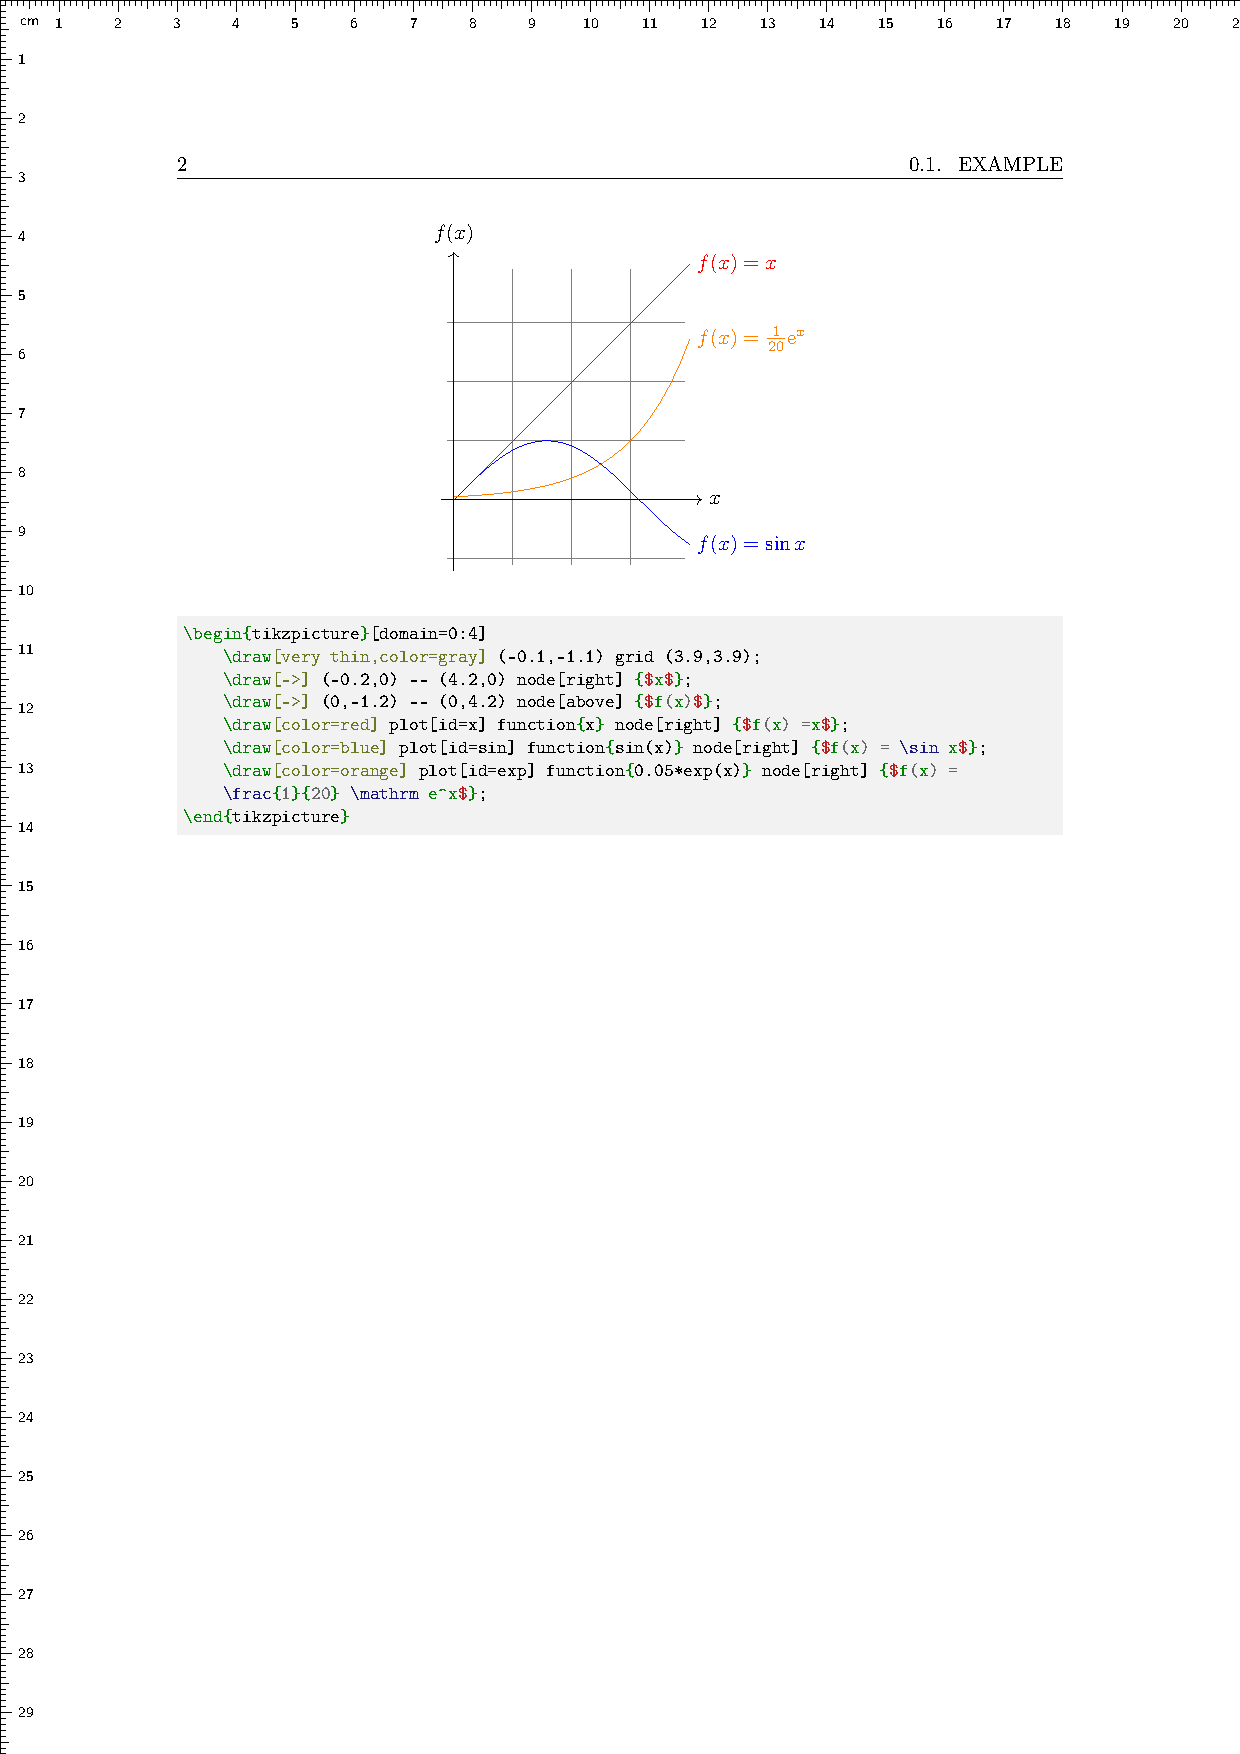
\includegraphics[width=.45\linewidth]{fgruler_2.pdf}
    \caption{页面布局示意图}
    \label{fig:fgruler-example}
\end{figure}

在设计本宏集时,我始终在字体配置上有所犹豫:是否应将字体打包进模板 ? 是否应在模板中为用户设置默认字体 ?
在本宏集的最初版本中,我尝试收集了一些免费的中英文字体,并直接放置在模板的文件夹中。然而,这种做法也带来了不少问题:

\begin{itemize}
    \item 部分用户真的需要该字体吗 ? 增加的字体会变成模板或用户的负担吗 ?
    \item 该字体可以随意传播吗 ? 万一某个用户将该字体进行了商用 ?
    \item 部分中文字体包含的字形往往是不全的, 怎么解决 ? 
    \item ...
\end{itemize}

最终的处理办法: 本宏集不打包任何的字体, 但添加部分 \TeX{}Live 内置字体配置; 宏集本身提供字体设置的接口, 但所有的字体定义
与样式由用户指定. 除此之外, \ztex{} 还提供了数学字体配置接口, 以供用户选用.

在开发 \ztex{} 宏集的过程中,行距等排版细节也曾让我困扰许久。实际上,设计一个模板需要考虑的因素远比预期复杂,几乎每一个
参数的设置都会相互影响。不过,在反复尝试与调整的过程中,我也逐渐总结出一条经验:对于一时把握不准的配置,就保留默认设置。

\textcolor{red}{Be simple, be fool} -- 保持简单,反而更容易达到稳定和谐的效果。

尽管在开发过程中遇到了诸多困难,\zTeX{} 最终仍未烂尾,顺利完成并呈现在了大家面前。


\clearpage
\subsection{无题}
时至今日,再次回头来看我的这个模板,我反而有了一些其他的感受. 一个模板到底需要给用户定制什么东西 ? 到底需要给用户
多大的自由空间(配置选项)? 如果你的配置选项过多,像 \href{https://www.ctan.org/pkg/koma-script}{koma-script}, 
\href{https://ctan.org/pkg/memoir}{Memoir} 那样, 模板作者给用户处理了很多的细节,提供了种类繁多的接口. 或者像部分简单
的模板仅提供几个必要的设置和命令; 而且,如果一个模板的说明文档都达到了上百页,那么我作为一个用户为什么不自己学习做模板,写一个
适合自己的模板,反而要话这部分时间来学习使用你的模板? 如果模板的配置选项过少,那么用户又会觉得这个模板不够灵活. 所以,
到底什么样的一个模板设计才能够称得上是:\textcolor{red}{\sffamily 简单,灵活,易用}? 遗憾的是,现在我也没有办法回答这个问题,所以这个问题作为习题,
留给使用者回答了 ...


发展至今,\ztex{} 宏集早已不再是一个简单的 ``文档类 + 绘图库 + 幻灯片'' 集合,这也使得它并不适合 \LaTeX{} 初学者使用。
在开发的过程中,我也逐渐意识到:很多时候,我们并不一定需要亲自设计一个模板。更合理的做法或许是 -- 根据自己的需求,选择合适的
功能性宏包,并通过它们提供的接口实现所需的功能。这种方式不仅更贴合实际使用场景,也减少了与其他宏包的兼容性问题,更无需投入
大量时间去理解第三方模板的结构与细节.

实际上,\cls{article}、\cls{book} 等基础文档类,加上丰富的功能宏包,已经足以满足绝大多数排版需求。也许我们并不需要再去重复造
一个模板的 ``轮子''。相比之下,我更认同将精力投入到基础性宏包的开发上,就如 \pkg{pgf}、\pkg{l3draw} 等优秀项目所做的那样 -- 它们
专注于提供一组底层的绘图或功能接口,将更高层的封装留给用户根据自身需求自行实现。

\vskip1em
\hfill\begin{tabular}{r}
  Happy \LaTeX{}ing ! \\
  \texttt{>\_<} \\
\end{tabular}





\clearpage
\section{文档指南}
\subsection{记号说明}
本宏集的所有用户手册均遵守如下规范:
\begin{itemize}
  \item 命令和键值对采用打字机字体;
  \item 键的默认值通过加粗标明, 并且与右侧蓝色文本一致;
  \item 所有命令排版格式为: \texttt {\textbackslash cmd [oArg]\{pArg\}};
  \item 所有键值排版格式为: \texttt{\zkey{key} = value};
\end{itemize}


\subsection{复制样例}
\ztex{} 宏集的所有用户手册均提供了大量示例及其对应的代码。为提升阅读体验,在排版过程中对部分代
码抄录环境中的符号进行了格式上的调整。例如:

\begin{itemize}
  \item 在示例代码中,换行符可能以 ``$\swarrow$'' 表示,复制代码时请将该符号删除;
  \item 若示例中包含行号,请在复制后手动去除多余的行号;
  \item 此外,在后续的 Implementation 节中,部分代码因排版原因进行了换行,使用时请根据实际情况去除不必要的换行符,
    以确保代码能够正确编译。 
\end{itemize}


\clearpage
\subsection{键值指定}
本系列中的大多数命令均采用键值对形式调用,因此,如果某个命令的可用键较多,而用户手册中的说明又较为模糊,用户可参考手
册末尾 Implementation 部分中该命令的声明原型。该部分列出了该命令所支持的所有键及其默认值,有助于进一步理解和正确
使用命令。下面以具体命令 \cmd{\Polygon} 为例,说明如何使用键值对接口:

\begin{texhigh}[]
% key-value setup
\keys_define:nn { ztikz / polygon }
  {
    radius       .fp_set:N  = \l__polygon_radius_fp,
    radius       .initial:n = { 1 },
    edgeColor    .tl_set:N  = \l__polygon_edge_color_tl,
    edgeColor    .initial:n = { black },
    fillColor    .tl_set:N  = \l__polygon_fill_color_tl,
    fillColor    .initial:n = { white },
    fillOpacity  .fp_set:N  = \l__polygon_fill_opacity_fp,
    fillOpacity  .initial:n = { 0 },
    rotate       .fp_set:N  = \l__polygon_rotate_angle,
    rotate       .initial:n = { 0 },
    shift        .tl_set:N  = \l__polygon_shift_tl,
    shift        .initial:n = { (0,0) },
    marker       .tl_set:N  = \l__polygon_marker_option_tl,
    marker       .initial:n = { },
  }
% command
\NewDocumentCommand\Polygon{ O{}m }
  {
    \group_begin:
    \keys_set:nn { ztikz / polygon } { #1 }
    ... 
    \group_end:
  }
\end{texhigh}

上述 \cmd{\Polygon}命令解读:它的第一个参数为一个可选参数(\cmd{O}类型), 通过键值对进行指定.
可用的键有: \zkey{radius}, \zkey{edgeColor}, \zkey{fillColor}, \zkey{fillOpacity}, \zkey{rotate}, 
\zkey{shift}, \zkey{marker}等. 其中键 \zkey{radius} 接受一个浮点数 (参考后面的:``\cmd{\fp_set:N}''), 默认值为
1(参考后面的:``\cmd{.initial:n = { 1 }}''); 再比如, 键 \zkey{edgeColor} 可以接受一个 tokenlist(参考后面的:``\cmd{\tl_set:N}''), 
默认值为 ``black'' (参考后面的:``\cmd{.initial:n = { black }}'').

\end{document}